\documentclass[
hyperref={pdfpagelabels=false}
%,red %, notes=show
,xcolor=table
% ,handout % UNCOMMENT FOR HANDOUT - also uncomment \pgfpagesuselayout
]
{beamer}

%\usecolortheme{beaver}


\setlength {\marginparwidth }{2cm}
\usepackage{todonotes}

\definecolor{Myred}{rgb}{0.7, 0.2, 0.2}

\usecolortheme[named=Myred]{structure}


\newcommand{\plus}{{
\includegraphics[scale=0.01]{plus.png}}}
\newcommand{\minus}{{
\includegraphics[scale=0.06]{minus.png}}}

\usepackage{pres}
% \usepackage{mathdots}
%\usepackage{qtree}
\usepackage{pgfpages}
% \pgfpagesuselayout{4 on 1}[a4paper, landscape,border shrink=5mm]
%\pgfpagesuselayout{2 on 1}[a4paper,border shrink=5mm]
\pgfpageslogicalpageoptions{1}{border code=\pgfusepath{stroke}}
\pgfpageslogicalpageoptions{2}{border code=\pgfusepath{stroke}}
\pgfpageslogicalpageoptions{3}{border code=\pgfusepath{stroke}}
\pgfpageslogicalpageoptions{4}{border code=\pgfusepath{stroke}}

\usepackage{picture}
\usepackage{pgfplots}
\usepackage{filecontents}
% \pgfplotsset{compat=1.12}
\usepackage{pdflscape}

\beamertemplatenavigationsymbolsempty

\newcommand{\travail}{\textbf{ICI IL Y A D TRAVAIL!}}

%%%%%%%%%%%%%%%%%%%%%%%%%%%%%
%%%%% PRESENTATION INFO %%%%%
%%%%%%%%%%%%%%%%%%%%%%%%%%%%%
\title[CSC - Intro]{Cryptography - Principles \\ --Cryptographie et Sécurité des Communications--} 
\author[]{Lionel Morel}
\institute[]{Telecommunications - INSA Lyon}
\date{Fall-Winter 2021-22}


%%%%%%%%%%%%%%%%%%%%%%%%%
%%%%%%%% COLORS %%%%%%%%%
%%%%%%%%%%%%%%%%%%%%%%%%%
\definecolor{greenCiti}{RGB}{83,186,89}
\definecolor{darkGreen}{RGB}{60,132,136}
\definecolor{purple}{RGB}{76, 69, 164}
\colorlet{corecolor}{lightgray}
\definecolor{uncorecolor}{RGB}{222,181,182}
\definecolor{lightgray}{rgb}{0.8,0.8,0.8}
\definecolor{lightblue}{RGB}{188,212,244}
\colorlet{socketcolor}{blue!20}

\colorlet{getpcolor}{red}
\colorlet{leetcolor}{darkGreen}

\definecolor{redfixit}{RGB}{188,43,0}
\definecolor{yellowfixit}{RGB}{235,237,62}
\definecolor{bluefixit}{RGB}{7,2,236}
\definecolor{orangefixit}{RGB}{227,118,24}
\definecolor{cyanfixit}{RGB}{1,171,159}
\definecolor{purplefixit}{RGB}{206,92,232}
\definecolor{greenfixit}{RGB}{102,156,52}



\AtBeginSection[]{
    \begin{frame}
    \vfill
    \centering
    \begin{beamercolorbox}[sep=8pt,center,shadow=true,rounded=true]{section page}
        \usebeamerfont{title}%
        {\color{Myred} \Huge \insertsectionhead}\par
    \end{beamercolorbox}
    \vfill
    \end{frame}
}


\usepackage{tcolorbox}
\tcbset{colframe=white,colback=white,nobeforeafter}




\begin{document}

\begin{frame}
  \maketitle
\end{frame}

\section{Context}

\begin{frame}
  \frametitle{Cryptographie}
\end{frame}


\begin{frame}
  \frametitle{Objectives}

  \begin{itemize}
  \item Encryption / Decryption (Confidentiality)
  \item Verification (Integrity)
  \item Signature (Authenticity)
  \end{itemize}
\end{frame}

\begin{frame}
  \frametitle{One-Time Pads}

  \begin{itemize}
  \item On se souvient de comment ça marche.
  \item On se souvient des limites principales:
    \begin{itemize}
    \item la clé (l'OTP) doit être aussi grande que le message.
    \item Générer du ``Vrai'' random c'est dur. 
    \end{itemize}
  \item On fait remarquer qu'une force des OTPs qu'on veut
    ``retrouver'' (même si un peu moins forte) c'est que le chiffré ne
    doit pas faire ressortir de ``régularité statistique'' du
    plaintext.
  \end{itemize}
\end{frame}


\begin{frame}
  \frametitle{One-Time Pads}

  On se souvient par contre que le One-Time Pad est ``parfait'' en terme de sécurité. On va donc chercher à construire des crypto-systèmes qui soient ``également'' parfaits.

  D'abord on définit les propriétés de telles systèmes: Kerchoffs et Shannon
  
\end{frame}


\begin{frame}
  \frametitle{Kerchoffs Principle {\normalsize (in ``La Cryptographie Militaire'' 1883)}}
  \begin{center}
    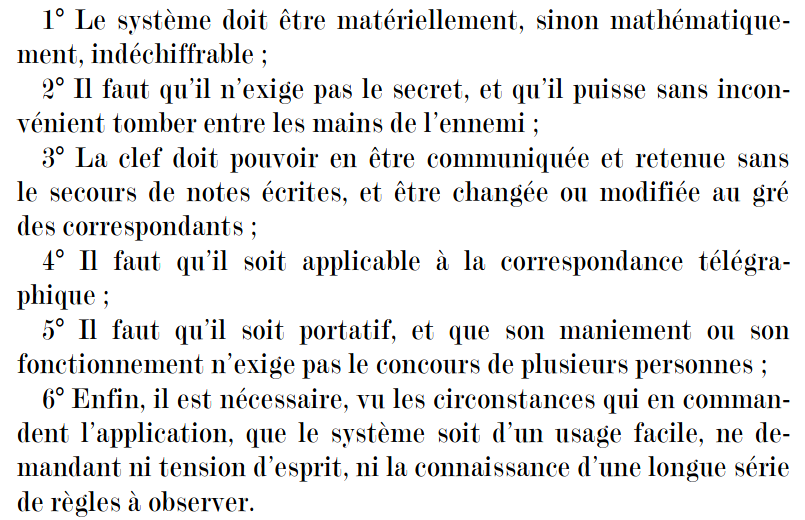
\includegraphics[width=\textwidth,height=0.5\textheight,keepaspectratio]{Kerckhoffs.pdf}
  \end{center}
  
  \begin{itemize}
  \item The adversary knows the system [Shannon]
  \item $\ne$ Security by Obscurity
  \item Largely accepted in cryptography
  \item Can be more widely applied to InfoSec (Information System Security) in general. 
  \end{itemize}
\end{frame}


\begin{frame}
  \frametitle{Confusion and Diffusion (Shannon, 1949)}

  \begin{block}{Confusion}
    \begin{itemize}
    \item Each bit in the ciphertext should \textbf{depend on several parts of
      the key}
    \item Usually implemented using \textbf{Substitutions}, aka S-Boxes
    \end{itemize}
  \end{block}


  \begin{block}{Diffusion}
    \begin{itemize}
    \item Encryption/decryptions imply an \textbf{avalanche effet}. Formally (in the original Shannon description): changing a single bit in the plaintext changes half of the bits in the cipher-text (eg at the block granularity)
    \item Usually implemented using \textbf{Permutations} (P-Boxes)
    \end{itemize}
  \end{block}
  
\end{frame}



\begin{frame}
  \frametitle{Precautions}

  \begin{itemize}
  \item Use recognized libraries (eg OpenSSL), not your own implementation
  \item Prefer open-source implementations (easier to identify bugs and backdoors)\footnote{\url{https://www.theguardian.com/world/2013/sep/05/nsa-how-to-remain-secure-surveil}lance}
  \item In this class, a lot of simplified versions (same on wikipedia)
  \item 
  \end{itemize}

  
\end{frame}

\section{Symmetric Encryption}


\begin{frame}
  \frametitle{Symmetric Cryptography - Principles}

  \begin{center}
    \includegraphics[width=\textwidth]{symCrypto-basic.pdf}
  \end{center}

  \begin{itemize}
  \item Encryption, Decryption, Signature and Verification use the same key
  \item Used implementations are quite efficient. 
  \item A key for each pair of communicating entities
  \item[$\Rightarrow$] Rapid explosion in the number of keys
  \end{itemize}
\end{frame}


\begin{frame}
  \frametitle{Symmetric ciphers - Basic Principles}

  \begin{center}
    \includegraphics[width=\textwidth,height=0.6\textheight,keepaspectratio]{fig/subPerm-principle.pdf}
  \end{center}
  
  Built as a network of substitution/permutation functions:
  \begin{itemize}
  \item Substitution: replace $n$ bits by a pre-determined (but moving) table. Must be one-to-one (to allow reversibility of encryption function)
  \item Permutation: exchange bits
  \end{itemize}
 
\end{frame}

\begin{frame}
  \frametitle{Symmetric ciphers - Baisc Principles}

  \begin{block}{Block cipher}
    \begin{itemize}
    \item Treat input as fixed-size blocks (between 64 and 128 bits)
    \item[\plus] More secure
    \item[\minus] Requires padding
    \end{itemize}
  \end{block}


  \begin{block}{Stream cipher}
    \begin{itemize}
    \item Treat input one byte at a time
    \item[\plus] fast HW implementation
    \item[\minus] Security less guaranteed
    \end{itemize}
  \end{block}
\end{frame}

\begin{frame}
  \frametitle{Symmetric ciphers - Basic Principles}

  Operation Modes:
  \begin{itemize}
  \item Electronic Code Book
  \item Cipher Block Chaining
  \item CounTeR
  \end{itemize}

  \textbf{TODO: expliquer chacun dans les grandes lignes}
  
\end{frame}





\begin{frame}
  \frametitle{Feistel}
  \begin{minipage}{.35\linewidth}
    \includegraphics[width=\textwidth]{Feistel.pdf}
  \end{minipage}
  \begin{minipage}{.55\linewidth}
    \begin{itemize}
    \item block cipher
    \item $r$ rounds
    \item key $k$ is spilt into $r$ subkeys: $(k_0, ..., k_{r-1})$
    \item plaintext = $(L_0, R_0)$
    \item $(L_{i+1}, R_{i+1}) = (R_i, L_i \oplus f_{k_i}(R_i))$
    \end{itemize}
  \end{minipage}
\end{frame}


\begin{frame}
  \frametitle{Feistel - Weaknesses and Attacks}

  \textbf{TODO}
  
\end{frame}

\begin{frame}
  \frametitle{Symmetric Cryptography - DES}

  Expands Feistel algorithm, by introducing: 
  \begin{itemize}
  \item More permutations
  \item Substitution Boxes (S-Boxes)
  \end{itemize}

  
  \begin{itemize}
  \item Designed (and initially published) in 1975.
  \item Block-cipher
  \end{itemize}

\end{frame}


% \begin{frame}
%   \frametitle{S-Boxes}


%   \textbf{Redondant!!}
  

%   \begin{itemize}
%   \item Obscure the relationship between the key and the ciphertext
%   \item m-bits input $\longrightarrow$ n-bits output
%   \item Implemented as a lookup table (efficient)
%   \end{itemize}

%   \begin{center}
%     \includegraphics[width=\textwidth,keepaspectratio]{fig/example-Sbox.png}
%   \end{center} 
 
% \end{frame}


\begin{frame}
  \frametitle{DES - General Algorithm}
  \begin{center}
    \includegraphics[height=0.8\textheight,keepaspectratio]{fig/DES1.pdf}
  \end{center} 
  
\end{frame}

\begin{frame}
  \frametitle{DES - One Round}
  \begin{center}
    \includegraphics[height=0.8\textheight,keepaspectratio]{fig/DES-OneRound.pdf}
  \end{center} 

\end{frame}


\begin{frame}
  \frametitle{DES - Weaknesses and Attacks}

  \begin{itemize}
  \item Most practical attack to date: still brute force (ie trying out all possible key in turn).
  \item Key size in DES was reduced from 128 bits to 56 bits (after discussions with ... NSA) ``to fit on a single chip''
  \item Practically cracked (brute-forced) in 1997
  \item Attacks faster than brute-force:
    \begin{itemize}
    \item Differential cryptanalysis: requires $2^{47}$ chosen plaintexts
    \item Linear cryptanalysis: requires $2^{43}$ chosen plaintexts
    \item TODO: explain each. 
    \end{itemize}
  \end{itemize}
\end{frame}


\begin{frame}
  \frametitle{Differential Cryptanalysis}

  \textbf{A FINIR}

  
  Principle: 
  \begin{itemize}
  \item Choose two plaintexts $x$ and $y$ such that: \\
    $y = x \oplus \Delta_x$
  \item Compute the corresponding cyphertexts and for each S-Box S: 
    \begin{itemize}
    \item $S(x)$
    \item $S(y) = S(x \oplus \Delta_x)$
    \end{itemize}
  \item Compute difference on S-Boxes:
    \begin{itemize}
    \item $\Delta_y = S(x \oplus \Delta_x) \oplus S(x)$
    \end{itemize}
  \item Repeat this for many plaintexts and several key hypothesis $k_i i \in \{0, n\}$
  \end{itemize}
\end{frame}


\begin{frame}
  \frametitle{Linear Cryptanalysis}

  \textbf{A FAIRE}
  
\end{frame}


\begin{frame}
  \frametitle{3DES}

  \begin{itemize}
  \item Standardized in 1998 to compensate for the weaknesses of DES
  \item DES has a 56-bits key
  \item 3DES chains 3 DES together:
    \begin{itemize}
    \item Encrypt(K1)$\rightarrow$Decrypt(K2)$\rightarrow$Encrypt(K1)
    \item Decrypt(K1)$\rightarrow$Encrypt(K2)$\rightarrow$Decrypt(K1)
    \item Key: 112 bits (K1 + K2)
    \end{itemize}
  \item Developped in parallel of AES (waiting for AES to be defined)
  \end{itemize}
 
\end{frame}




\begin{frame}
  \frametitle{AES - Advanced Encryption Standard}
  \begin{itemize}
  \item Supersedes DES
  \item Standardized in 2001
  \item NIST-organized competition with 5 finalists:
    \begin{itemize}
    \item IBM proposed MARS
    \item RSA proposed RC6
    \item Serpent by Anderson, Bihman, Knudsen
    \item Twofish by Cruce Schneier et al
    \item Rijndael, by Daemen and Rijmen
    \end{itemize}
  \item Rijndael's was elected by community after a thourough international comparative effort (including NSA, companies, academics), based on security, performance (speed, memory usage).
  \item NB: no-patent allowed (imposed by the NIST)
  \end{itemize}
\end{frame}


\begin{frame}[fragile]
  \frametitle{Algorithm}
\begin{minted}{C}
void AES_Run_secure(void){
  int i;
  addRoundKey();
  for(i = 0; i < 9; i++){
      subBytes();
      shiftRows();
      mixColumns();
      computeKey(rcon[i]);
      addRoundKey();
  }
  subBytes();
  shiftRows();
  computeKey(rcon[i]);
  addRoundKey();
}
\end{minted}
\end{frame}




\begin{frame}[fragile]
  \frametitle{AES explained\footnote{\url{https://en.wikipedia.org/wiki/Advanced_Encryption_Standard}}}

  \begin{itemize}
  \item \textbf{KeyExpansion} --- round keys are derived from the
    cipher key using the AES key schedule. AES requires a separate
    128-bit round key block for each round plus one more.
  \end{itemize}
\end{frame}



\begin{frame}[fragile]
  \frametitle{AES (cont'd)}
  \begin{itemize}
  \item \textbf{Initial round key addition}:

    \begin{itemize}
    \item \textbf{AddRoundKey} – each byte of the state is combined with a byte
      of the round key using bitwise xor.
    \end{itemize}
  \end{itemize}

  \begin{center}
  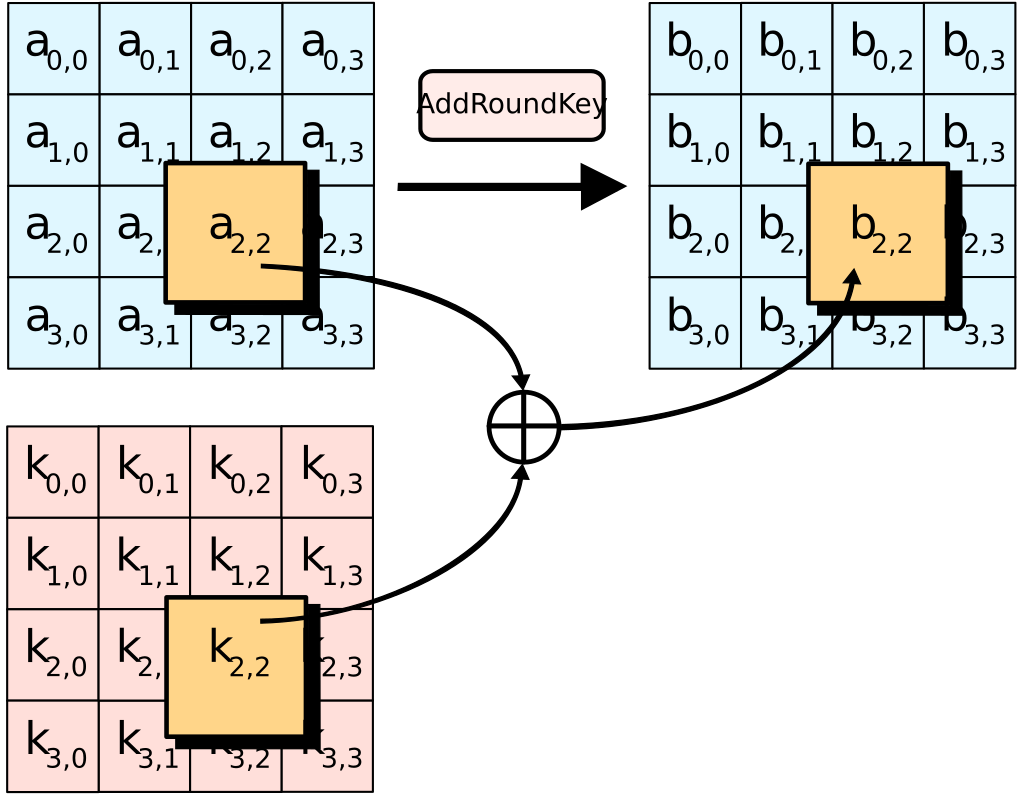
\includegraphics[width=\textwidth,height=0.6\textheight,keepaspectratio]{AES-AddRoundKey.png}
\end{center}
  
  
\end{frame}



\begin{frame}
  \frametitle{AES - SubBytes}

  SubBytes = a non-linear substitution step where each byte is
  replaced with another according to a lookup table.

  \begin{center}
    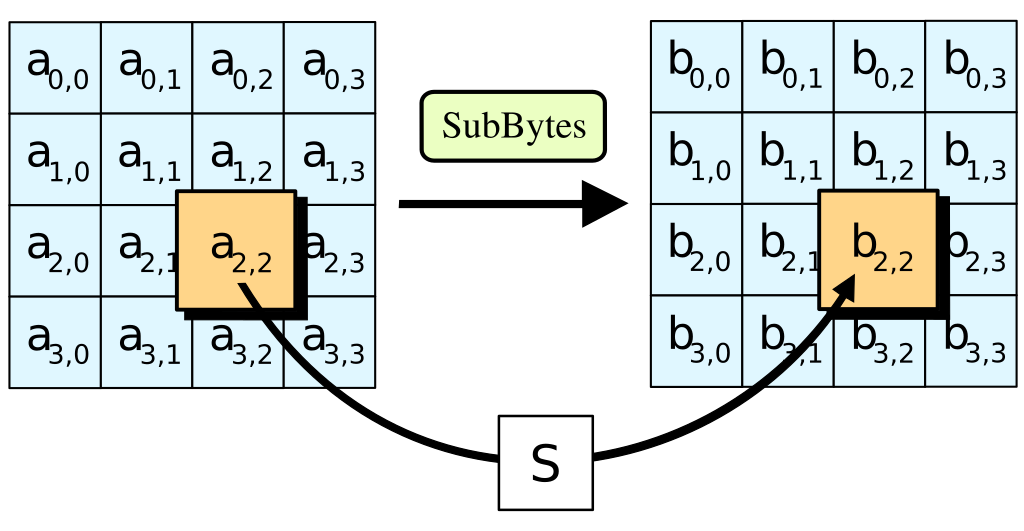
\includegraphics[width=\textwidth,height=0.6\textheight,keepaspectratio]{AES-SubBytes.png}
  \end{center}
 
\end{frame}


\begin{frame}
  \frametitle{ShiftRows}
  ShiftRows = a transposition step where the last three rows of the state are shifted cyclically a certain number of steps.  


  \begin{center}
    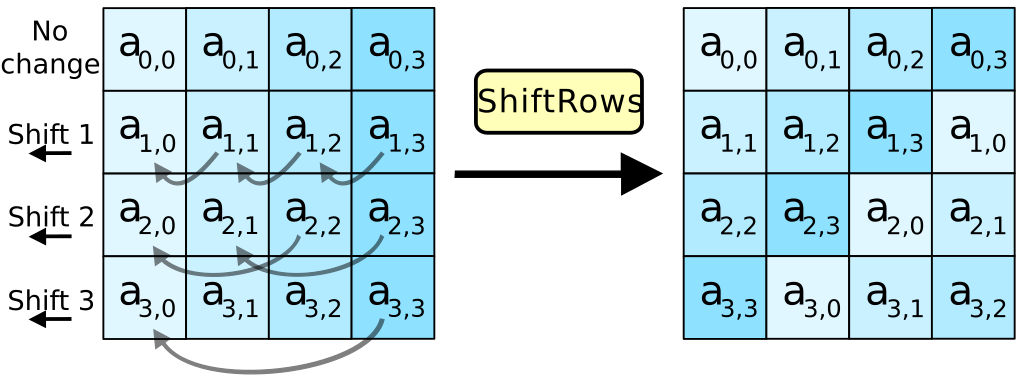
\includegraphics[width=\textwidth,height=0.6\textheight,keepaspectratio]{AES-ShiftRows.png}
  \end{center}
 
\end{frame}


\begin{frame}
  \frametitle{MixColumns}
  MixColumns = a
      linear mixing operation which operates on the columns of the
      state, combining the four bytes in each column.
      AddRoundKey


  \begin{center}
    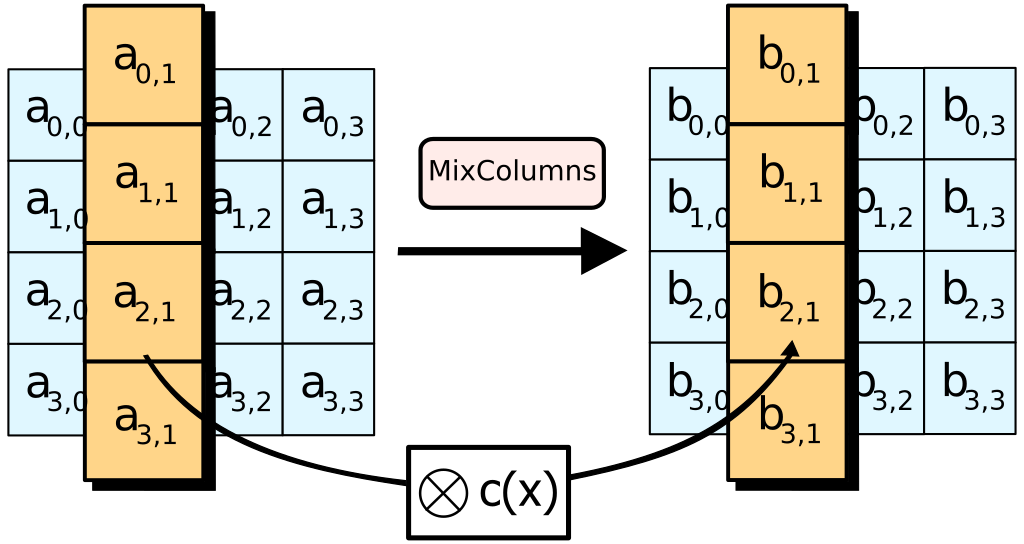
\includegraphics[width=\textwidth,height=0.6\textheight,keepaspectratio]{AES-MixColumns.png}
  \end{center}
 
\end{frame}

\begin{frame}
  \frametitle{AES - Weaknesses and Attacks}

  \textbf{TODO}
  
\end{frame}



\begin{frame}
  \frametitle{Symmetric Cryptogaphy - Conclusions}

  \begin{itemize}
  \item[\plus] Overall very effecient (linear in the size of data to encrypt)
  \item[\plus] Arithmetic/Logical operations are simple: xor. 
  \item[\minus] Requires a shared key! 
  \item Solutions to this:
    \begin{itemize}
    \item Avoid the need for a common key
    \item Find a way to securely share a common key
    \end{itemize}
  \end{itemize}
\end{frame}


\begin{frame}
  \frametitle{Aparté}

  Expliquer qu'il y a des ``secret key storage'' en HW, des trucs inviolables où un fabricant peut installer des clés à l'usine. (mais bon, y a de toute façon la question de la chain of trust). voir \url{https://en.wikipedia.org/wiki/Chain_of_trust}
\end{frame}



\begin{frame}
  \frametitle{Key Sharing Problem}
  
\end{frame}


\begin{frame}
  \frametitle{Diffie-Hellman Key Exchange}
  \begin{center}
    \includegraphics[width=\textwidth,height=0.7\textheight,keepaspectratio]{fig/DiffieHellman.pdf}
  \end{center}
\end{frame}



\section{Hash}


\begin{frame}
  \frametitle{Cryprographic Hash}


  \begin{center}
    \includegraphics[width=\textwidth]{hmac.pdf}
  \end{center}
  
  \begin{itemize}
  \item eg Hash-based Message Authentication Code
  \item Only sender and recipient can sign/verify the message
  \end{itemize}
  
\end{frame}

\begin{frame}
  \frametitle{Cryptographic Hash - Principle}

  \begin{itemize}
  \item Compute a ``footprint''
  \item The message can be of any size, the footprint is of fixed size
  \item Pseudo-unique identification of message
  \item Used for:
    \begin{itemize}
    \item Integrity checks
    \item Cryptographic signature
    \item PRNG
    \item Hashed password storage
    \end{itemize}
  \end{itemize}
\end{frame}


\begin{frame}
  \frametitle{Cryptographic Hash - Good Properties}

  \begin{itemize}
  \item \textbf{Pre-image resistance}: no one can reverse the hash function (to find input from output)
  \item \textbf{Second pre-image resistance}: unicity of hash. Given an input and the corresponding hash, one cannot find another input with the same hash. 
  \item \textbf{Collision-resistance}: no-one can produce two different inputs with the same hash
  \item \textbf{Randomness}
  \end{itemize}
\end{frame}


\begin{frame}
  \frametitle{Cryptographic Hash - today' state of affairs}

  Existing (and used) implementations
  \begin{itemize}
  \item MD5: please don't use anymore: ``cryptographically broken and
    unsuitable for further use''
  \item SHA-1: not recommanded anymore (since 2017)
  \item SHA-2: still not planned for removal
  \item SHA-3: standardized in 2015
  \end{itemize}

  Current situation:
  \begin{itemize}
  \item Hash functions are critical in crypto!
  \item SHA-2 is still safe but is conceptually close to SHA-1 and might share some weaknesses with it
  \item SHA-3 considered ``as safe'' but built completely differently
  \end{itemize}
\end{frame}

\section{Asymmetric Cryptography}



\begin{frame}
  \frametitle{(general) Asymmetric Cryptography}

  \begin{itemize}
  \item Each participant $u$ has a pair of keys $Pub_u$ and $Priv_u$. 
  \item $u$ sends $Pub_u$ to $v$
  \item $v$ sends $Pub_v$ to $u$
  \item $u$ can encrypt its messages to $v$ using a combination of $Pub_v$ and $Priv_u$
  \item $v$ can decrypt messages from $u$ using a combination  of $Pub_u$ and $Priv_v$
  \end{itemize}

  Note:
  \begin{itemize}
  \item Relies on ``hard mathematical problems'':
    \begin{itemize}
    \item Discrete logarithm
    \item Factorization of large numbers
    \end{itemize}
  \item Usually slow (exponentiation)
  \end{itemize}
\end{frame}

\begin{frame}
  \frametitle{RSA}
  \begin{itemize}
  \item Invented in 1977 by Rivest, Shamir and Adleman
  \item MIT Patent in 1983, expired in 2000
  \item Security based on the difficulty of factorizing large integers
  \end{itemize}
\end{frame}


\begin{frame}
  \frametitle{RSA - Key generation}

  \begin{itemize}
  \item Choose $p$ and $q$, two prime numbers: random, kept secret
  \item Compute $n = pq$
  \item Compute $\lambda(n)$,
    \begin{itemize}
    \item $\lambda(n) = lcm(\lambda(p), \lambda(q))$
    \item $= lcm(p-1, q-1)$
    \item $= \frac{pq}{gcd(p,q)}$ ... (gcd obtained with Euclid. algorithm)
    \end{itemize}
  \item Choose $e$ s.t.:
    \begin{itemize}
    \item $1 < e < \lambda(n)$
    \item $gdc(e,\lambda(n))=1$
    \end{itemize}
  \item Compute $d = e^{-1} \mbox{ mod } \lambda(n)$
    \begin{itemize}
    \item $d$ is the ``private key exponent''
    \end{itemize}
  \end{itemize}

  \begin{tcolorbox}[colframe=Myred]
    $Pub = (e,n)$ \hfill $Priv = (d,n)$
  \end{tcolorbox}  
\end{frame}


\begin{frame}
  \frametitle{RSA - Encryption}

  \begin{center}
    \includegraphics[width=\textwidth,height=0.6\textheight,keepaspectratio]{fig/RSA-encryption.pdf}
  \end{center}
  
\end{frame}


\begin{frame}
  \frametitle{RSA - Decryption}

  \begin{center}
    \includegraphics[width=\textwidth,height=0.6\textheight,keepaspectratio]{fig/RSA-decryption.pdf}
  \end{center}
\end{frame}


\begin{frame}
  \frametitle{RSA - Signing}

  \textbf{TODO}

  (cf slides François)
  
\end{frame}

\begin{frame}
  \frametitle{RSA - Example}
  \begin{enumerate}
  \item $p = 61$ and $q = 53$
  \item n = pq = 3233
  \item $\lambda(n) = lcm(p-1, q-1)$
  \item $= \lambda(3233) = lcm(60,52) = 780$
  \item Choose $1<e<780$ (coprime to $780$), eg $e=17$
  \item $d = e^-1 \mbox{ mod } \lambda(n)$
  \item $= 413$ (as $1 = 17 * 413 \mbox{ mod } 780$)
  \item Public key = $(e = 17, n = 3233)$
  \item $c(m) = m^{17} \mbox { mod } 3233$
  \item Private key = $(d = 413, m = 3233)$
  \item $m(c) = c^{413} mod 3233$
  \item $m = 65 \rightarrow c = 65^{17} \mbox{ mod } 3233 = 2790$
  \item $2790 \rightarrow m = 2790^{413} \mbox{ mod } 3233 = 65$
  \end{enumerate}
  
\end{frame}

\begin{frame}
  \frametitle{RSA - Properties \& Limitations}

  \begin{itemize}
  \item[\plus] Finding $d$ requires factorizing $n$: proven difficult (for $p$ and $q$ large)
  \item[\minus] Implementation is tricky : good PRNG, acceptable $e$ 
  \item[\minus] Relies on exponentiation which is \textbf{expensive} 
  \end{itemize}

  \textbf{TODO : expliquer pourquoi l'exponentiation est chere :) }
  
\end{frame}


\section{Hybrid Cryptography}

\begin{frame}
  \frametitle{Comparing Symetric / Asymetric cryptogaphy}

  \textbf{Slide 61 de François}
  
\end{frame}


\begin{frame}
  \frametitle{}

  \textbf{Slide 62 de François}

  
\end{frame}




\end{document}

  